% Created 2021-11-12 ven 12:32
% Intended LaTeX compiler: xelatex
\documentclass[a4paper]{article}
\usepackage{graphicx}
\usepackage{longtable}
\usepackage{wrapfig}
\usepackage{rotating}
\usepackage[normalem]{ulem}
\usepackage{amsmath}
\usepackage{amssymb}
\usepackage{capt-of}
\usepackage{hyperref}
\usepackage{minted}
\usepackage{fontspec}
\setmainfont{Cabin}
\usepackage[margin=1.25in]{geometry}
\usepackage{minted}
\author{Matteo Orlando}
\date{}
\title{Programming for Iot - Lab 4}
\hypersetup{
 pdfauthor={Matteo Orlando},
 pdftitle={Programming for Iot - Lab 4},
 pdfkeywords={},
 pdfsubject={},
 pdfcreator={Emacs 27.1 (Org mode 9.6)}, 
 pdflang={English}}
\begin{document}

\maketitle
\tableofcontents


\section{Introduction}
\label{sec:org82c4036}

\subsection{Data format}
\label{sec:org8f19d80}
In this lab we will try to develop different kind of sensor simulator
that use REST and MQTT.

Remember to lways use SenML as data format:

\begin{minted}{javascript}
{
        "bn": "http://example.org/sensor1/",
        "e": [
                {
                    "n": "temperature",
                    "u": "Cel",
                    "t": 1234,
                    "v":22.5
                }
             ]
    }
\end{minted}

\subsection{Hardware connection}
\label{sec:org009fb14}
To check that the sensor works fine you should connect the DHT 11 sensor as
shown in the picture below

\begin{center}
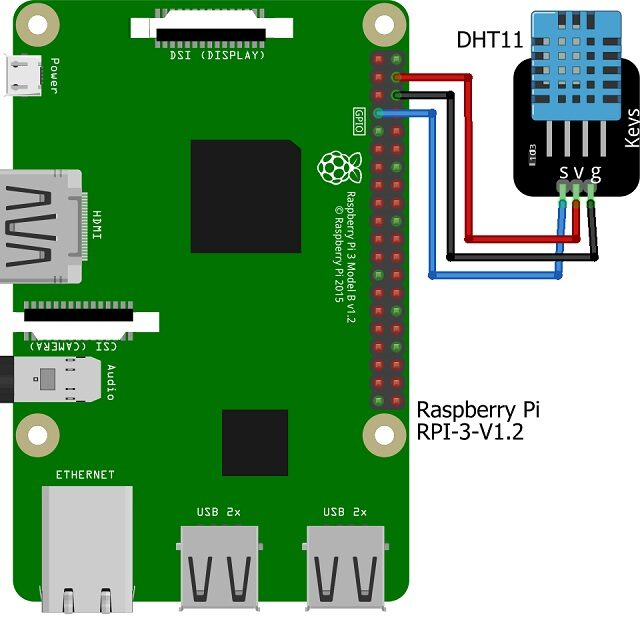
\includegraphics[width=7cm]{./images/dht11.jpg}
\end{center}

Then you should run the test file located in the ``Documents'' folder of the
Raspberry in order to check that the sensor is working.

\section{Exercices}
\label{sec:org9ca27ab}

\subsection{Exercise 1}
\label{sec:orgf6cd999}

Using the Raspberry Pi develop a REST service for the temperature sensor.
This sensor should provide a GET method to manage 3 different uri:

\begin{itemize}
\item ``/temperature'' should return the measured temperature as a json in SenML
format
\item ``/humidity'' should return the measured humidity in the as a json in SenML
format
\item ``/allSensor'' should return the data from all the sensor as a json in SenML
format
\end{itemize}

\textbf{Develop the script on your PC and check they work correctly on it before
deploying it on the Raspberry.}

\subsection{Exercise 2}
\label{sec:orgd05adad}

Using the Raspberry Pi develop an MQTT publisher and and MQTT subscriber
This publisher should publish every 5 seconds a message in SenML format with the
following information:

\begin{itemize}
\item ``/temperature'' should provide the measured temperature as a json in SenML
format
\item ``/humidity'' should provide the measured humidity in the as a json in SenML
format
\item ``/allSensor'' should provide the data from all the sensor as a json in SenML
format
\end{itemize}


The subscriber should be able to receive all the message from all the topics and
print it on screen in an user friendly way that indicates also the topic that
provide that message.

Example:
If the message below is received
\begin{minted}[breaklines=true,breakanywhere=true]{python}
    {
        "bn": "matteo/sensor1/temperature", 
        "e": [
                {
                    "n": "temperature", 
                    "u": "Cel", 
                    "t": 1234, 
                    "v":22.5 
                } 
             ]
    }
\end{minted}
The publisher should print
\begin{quote}
matteo/sensor1 measured a temperature of 22.5 Cel at the time 1234
\end{quote}

\textbf{Develop the script on your PC and check they work correctly on it before
deploying it on the Raspberry.}

When you're ready try to run the publisher on the raspberry and the subscriber
on your laptop to check if you developed a real IoT device.

\subsection{Exercise 3}
\label{sec:org4247f18}

In most of the cases we want to perform some kind of processing on the data we
receive to have more significant information to show to the user or to take
actions. In order to do this we need to develop script that are able to receive
data and process it according to our needs.

Therefore try to develop 2 post processing script as follow:

\begin{itemize}
\item The first one should ask the temperature to the sensor developed in the first
exercise every x seconds (choose x as you prefer, 3 should be a feasible
value). Every 10 data aquisition it should calculate the average temperature
and printing it on screen.
\item The second script should be an MQTT subscriber that will recieve the humidity
measurements from the sensor developed in the second exercise. Every 10
measurements it should publish a message with the average humidity at a topic
of your choice.
\end{itemize}

For the second script you can test that everything works using a subscriber with
a wildcard that prints all the message received.


\subsection{Exercise 4}
\label{sec:org642bb09}

In some cases, for testing reason it could be useful to have virtual sensors
that can emulate as much as possible the behaviour of a real one.

Develop an MQTT publisher to emulate an heartrate sensor that publish
random values in the range [55,180] every 5 seconds for 2 minutes.

Develop also an MQTT subscriber that receives these values, prints these
on screen and save these on a json file called \emph{hrLog.json}. To
generate the values, you can use one of the functions of the library
numpy listed at
\href{https://docs.scipy.org/doc/numpy-1.15.0/reference/routines.random.html}{this
link}, try with different functions to evaluate which is the one that
has the most realistic result. You can find a visualization of some of
this generator
\href{https://colab.research.google.com/drive/1JsxjaRDYnoMb6dQ5MZsLKH7ZDy7QzH9O?usp=sharing}{here}
(you can even make your test there before writing your code)


\subsection{Exercise 5}
\label{sec:org48924f3}

Develop an MQTT publisher to emulate a sensor of your choice that
publish random values in the 3 possible ranges. For example for an
heartrate sensor we could define 3 ranges as [resting,sport,danger].
Then create a simple terminal client for this MQTT publisher to select
the range to be used to send the data. Develop also an MQTT subscriber
to receive those data and in case of data in a warning range provide some kind
of feedback to the user.
\end{document}
